\section{anode Strukturreferenz}
\label{structanode}\index{anode@{anode}}
{\tt \#include $<$hashtab.h$>$}

Zusammengeh\"{o}rigkeiten von anode:\begin{figure}[H]
\begin{center}
\leavevmode
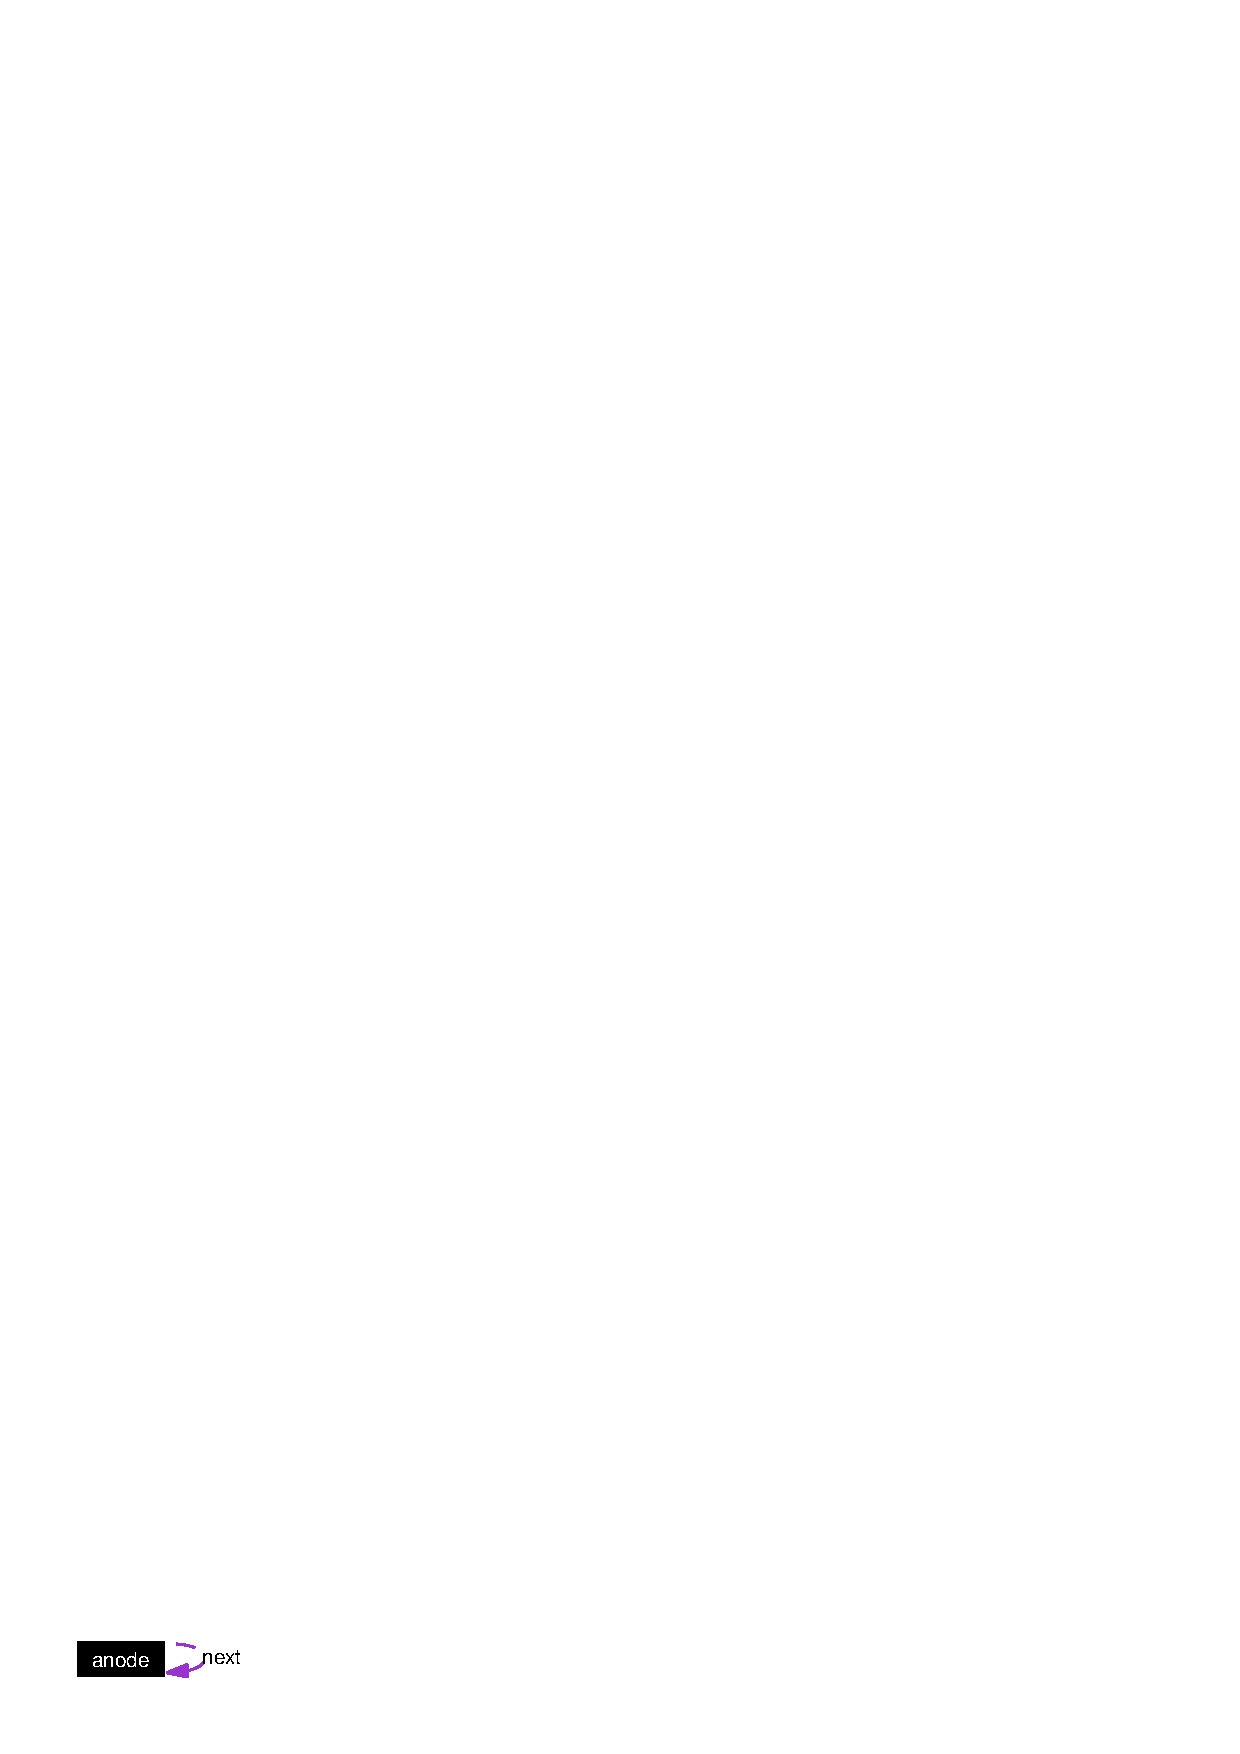
\includegraphics[width=59pt]{structanode__coll__graph}
\end{center}
\end{figure}
\subsection*{Datenfelder}
\begin{CompactItemize}
\item 
char $\ast$ {\bf string}
\item 
int {\bf flag}
\item 
u\_\-long {\bf count}
\item 
{\bf anode} $\ast$ {\bf next}
\end{CompactItemize}


\subsection{Ausf\"{u}hrliche Beschreibung}




Definiert in Zeile 50 der Datei hashtab.h.

\subsection{Dokumentation der Datenelemente}
\index{anode@{anode}!count@{count}}
\index{count@{count}!anode@{anode}}
\subsubsection{\setlength{\rightskip}{0pt plus 5cm}u\_\-long {\bf anode::count}}\label{structanode_358dd30d63b3ecf448451988c0139fcf}




Definiert in Zeile 52 der Datei hashtab.h.

Wird benutzt von all\_\-agents\_\-page(), dump\_\-all\_\-agents(), new\_\-anode(), put\_\-anode() und top\_\-agents\_\-table().\index{anode@{anode}!flag@{flag}}
\index{flag@{flag}!anode@{anode}}
\subsubsection{\setlength{\rightskip}{0pt plus 5cm}int {\bf anode::flag}}\label{structanode_f9635cb5d8af6707a8bfab885f6d556b}




Definiert in Zeile 51 der Datei hashtab.h.

Wird benutzt von all\_\-agents\_\-page(), dump\_\-all\_\-agents(), new\_\-anode(), put\_\-anode() und top\_\-agents\_\-table().\index{anode@{anode}!next@{next}}
\index{next@{next}!anode@{anode}}
\subsubsection{\setlength{\rightskip}{0pt plus 5cm}struct {\bf anode}$\ast$ {\bf anode::next}}\label{structanode_834db38618dba5e74b8a738441e861d9}




Definiert in Zeile 53 der Datei hashtab.h.

Wird benutzt von del\_\-alist(), load\_\-agent\_\-array() und put\_\-anode().\index{anode@{anode}!string@{string}}
\index{string@{string}!anode@{anode}}
\subsubsection{\setlength{\rightskip}{0pt plus 5cm}char$\ast$ {\bf anode::string}}\label{structanode_8fa6d7969583389ae6d535866f9fd914}




Definiert in Zeile 50 der Datei hashtab.h.

Wird benutzt von all\_\-agents\_\-page(), del\_\-alist(), dump\_\-all\_\-agents(), new\_\-anode(), put\_\-anode() und top\_\-agents\_\-table().

Die Dokumentation f\"{u}r diese Struktur wurde erzeugt aufgrund der Datei:\begin{CompactItemize}
\item 
oosalizer/{\bf hashtab.h}\end{CompactItemize}
